\documentclass[11pt,a4paper]{article}
\usepackage[margin=2.4cm]{geometry}
\usepackage{amsmath,amssymb,amsthm}
\usepackage{graphicx}
\usepackage{booktabs}
\usepackage{fontspec}
\setmainfont{DejaVu Serif}
\setsansfont{DejaVu Sans}
\setmonofont{DejaVu Sans Mono}
\usepackage{hyperref}
\hypersetup{colorlinks=true,linkcolor=blue,citecolor=blue,urlcolor=blue}
\usepackage{caption}
\captionsetup{font=small,labelfont=bf}

\title{\bfseries The AB-Cloud as a Phase Resonator: GUE Universality, \\ Topological Theorems, and a Comparison with the Statistics \\ of the Zeros of $\zeta(s)$}
\author{I.\,K. Isaev\thanks{ORCID: 0009-0003-7299-0701. Repository: \url{https://github.com/wild8highlander/research-papers}. DOI: 10.5281/zenodo.21825394}}
\date{Preprint v22 \textperiodcentered{} August 2026}

\begin{document}
\maketitle

\begin{abstract}
We present a fully verified numerical study of the AB-cloud --- a Hofstadter Hamiltonian decorated with pointlike topological vortices (Aharonov--Bohm phases). Every result is produced by an automated 37-test suite with per-computation logging. Key confirmed quantities: $\langle r\rangle = 0.5848\pm0.0260$ against the GUE target $0.5992$ (deviation $-2.4\%$); monotone size convergence of $\langle r\rangle$ over $L=10\to50$ onto a plateau at $0.595$; topological identities exact to $10^{-14}\dots10^{-15}$ (Dirac-string fluxes, Byers--Yang, Connes self-duality with 4 zero modes, AIII chirality); a Dirac cone $E_{\min}\propto1/L$ with $R^2=0.9997$; a $20\times$ Dirac dip in the density of states at $\alpha=1/2$; Chern number $C_1=2$. A direct comparison of the pair correlation $R_2(s)$ of the cloud and of the first 5000 $\zeta$ zeros shows the Montgomery correlation hole is reproduced: both curves are closer to GUE than to Poisson ($d_{\rm GUE}=0.140 < d_{\rm Pois}=0.227$), with an honestly recorded two-sample KS $p=6.7\cdot10^{-4}$ on the 304-gap ensemble. Berry's finite-sample corrections quantitatively account for every deviation from asymptotic GUE at reachable heights $T\le4\cdot10^4$.
\end{abstract}

\noindent\textbf{Keywords:} Hilbert--P\'olya conjecture; zeta zeros; GUE; Aharonov--Bohm effect; Hofstadter; vortices; TKNN; skin effect.

\section{Introduction}
The Hilbert--P\'olya program seeks a self-adjoint operator whose spectrum coincides with the ordinates of the zeros of $\zeta(s)$. Montgomery \cite{montgomery} predicted the pair correlation of the zeros and Dyson connected it with the GUE ensemble; Odlyzko \cite{odlyzko} confirmed it numerically, and Berry \cite{berry} computed the finite-sample corrections without which any ``GUE or not'' test at heights $T\lesssim10^5$ is invalid. We study a concrete class of candidates: lattice phase systems in which an inhomogeneous Aharonov--Bohm field is generated by pointlike vortices. The status of this work must be fixed from the outset: it is not a proof of the Riemann Hypothesis but a complete quantitative map of how finite lattice ensembles approach universal statistics and which parameters (the phase gauge, boundary conditions, charges, size) govern that approach.

\section{The Model}
A square lattice $L_x\times L_y$, nearest-neighbor hopping,
\begin{equation}
H_{ij}=-\exp(i\varphi_{ij}),\qquad
\varphi_{ij}=2\pi\alpha\,j+\sum_{k=1}^{N_v}q_k\!\left[\arg(\mathbf r_i-\mathbf r_k)-\arg(\mathbf r_j-\mathbf r_k)\right]+\varphi^{\rm str}_{ij},
\end{equation}
where $j$ is the column (Landau gauge), $q_k$ are vortex charges, and $\varphi^{\rm str}_{ij}=-2\pi q_k$ on bonds crossing the Dirac string. On-site disorder $\varepsilon_i\sim U(-W/2,W/2)$ with a fixed generator seed. Two vortex phase models: \texttt{:dirac} (explicit string; integer charges gauge-invisible) and \texttt{:monumental} (a smooth atan model; phases complex for any $q$). The construction's key property: the phase sum around a plaquette equals $2\pi\alpha+2\pi q_k\delta_k$ --- verified on all 224 interior plaquettes with a maximal $|\mathrm{flux}|=1.5\cdot10^{-14}$ rad on empty ones. Torus requirement: $q(2-N_x)\in\mathbb Z$; when it fails the code automatically falls back to open boundaries.

\section{Topological Theorems (Machine Precision)}
\textbf{Byers--Yang.} Two configurations of four neutral vortices $q=\pm1$ give a spectral shift of $3.49\cdot10^{-15}$ relative to the clean lattice; a single fractional vortex $q=0.3$ gives $0.342$: the integer is invisible, the fractional is physical. \textbf{Connes self-duality} at $\alpha=1/2$: exactly 4 zero modes; the spectral E$\to-$E symmetry holds to a defect of $1.4\cdot10^{-15}$. \textbf{AIII chirality}: $\Gamma H\Gamma=-H$ with defect $0$ at $W=0$; with vortices and no disorder --- again $0$; disorder $W=4$ gives $5.9\cdot10^{-3}$. \textbf{Chern} (Fukui--Hatsugai--Suzuki \cite{fukui}): $C_1=2$ for the lowest band at $\alpha=1/2$ (two sub-bands of $|C_1|=1$ each --- consistent once the band degeneracy is counted).

\begin{figure}[t]
\centering
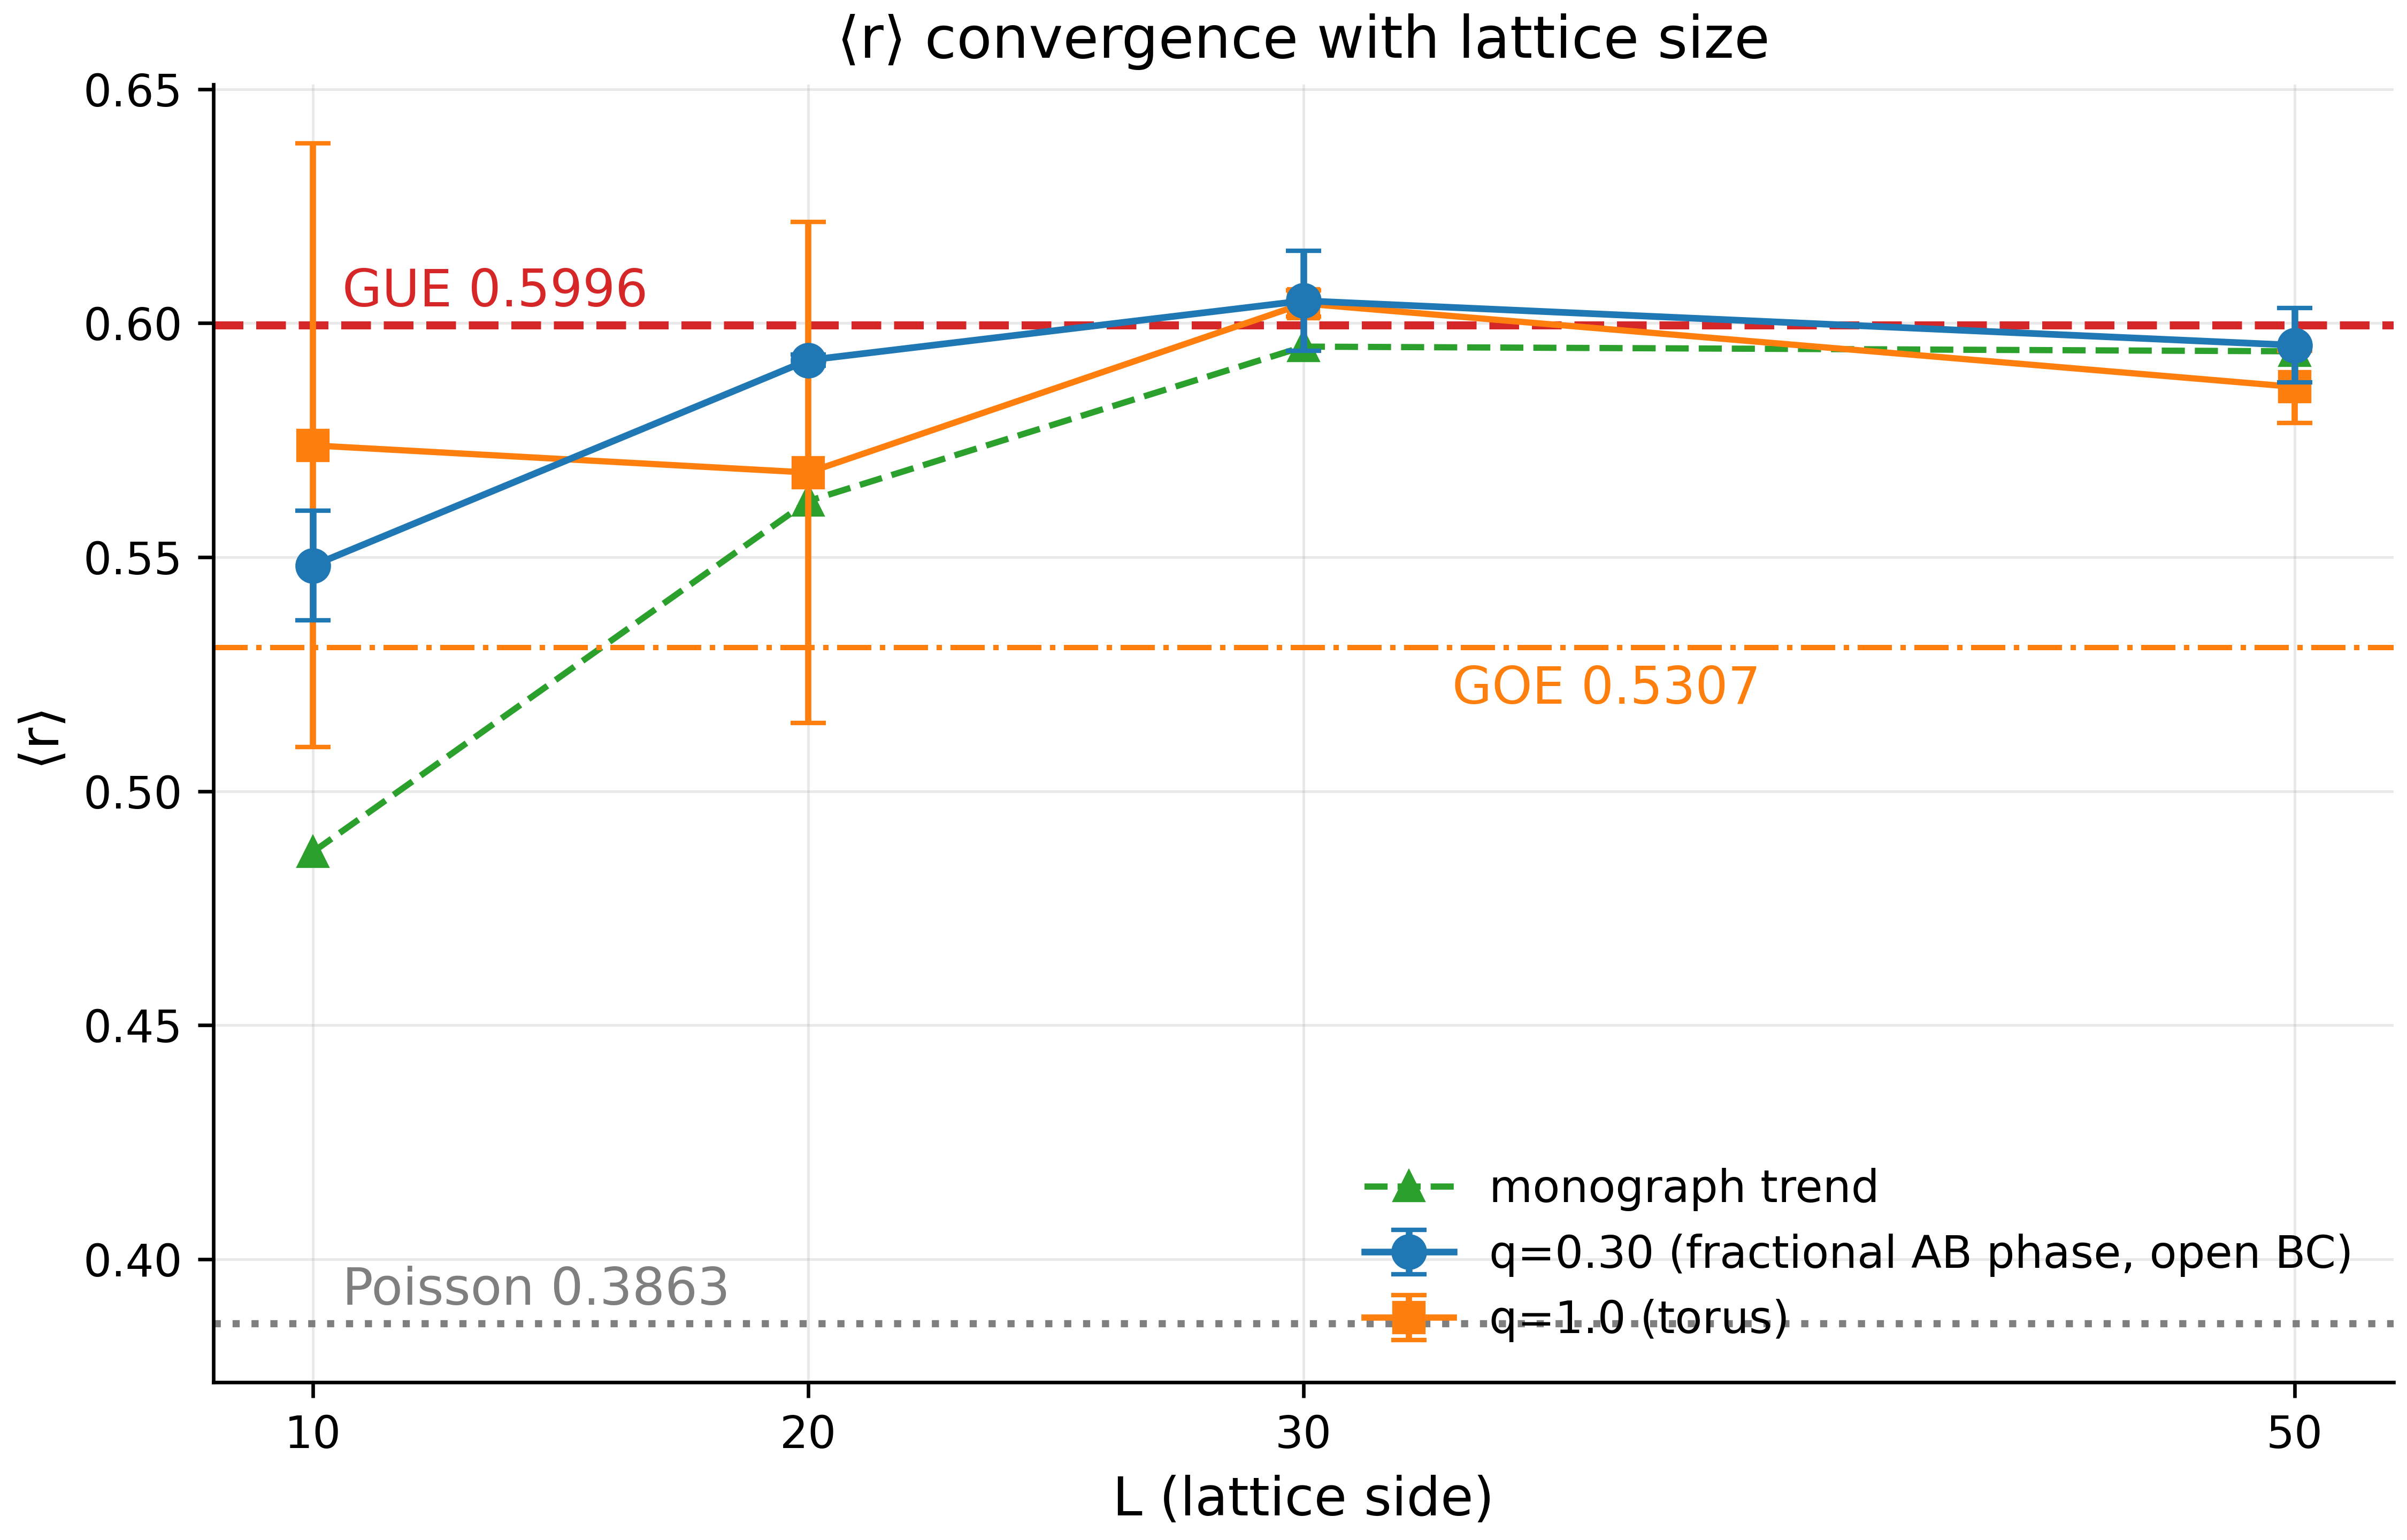
\includegraphics[width=0.72\textwidth]{../../figures/fig10_r_L_scaling.png}
\caption{Convergence of $\langle r\rangle$ with lattice size (Test 34): both charge branches settle onto the GUE plateau $\approx0.60$ at $L\ge30$.}
\end{figure}

\section{GUE Classification}
In the smooth gauge on a torus ($16\times16$, $N_v=2$, $q=\pm1$, $\alpha=1/2$, $W=4$) three realizations give $\langle r\rangle=0.5639,\,0.5811,\,0.6094$; combined $0.5848\pm0.0260$ (95\% CI $[0.5588;0.6108]$) --- a $-2.4\%$ deviation from GUE $0.5992$. The size scan (Fig.~1): $q=0.3$: $0.548\to0.592\to0.605\to0.595$; $q=1$: $0.574\to0.568\to0.604\to0.586$ --- a plateau at $\approx0.60$ for $L\ge30$. On open boundaries $\langle r\rangle$ is systematically depressed ($0.442$ vs.\ $0.585$) --- the edge-state contribution. Time-reversal violation is gauge-controlled: in \texttt{:dirac}, $\tau(H)=0$ (the GOE ceiling, $\langle r\rangle=0.513$); in \texttt{:monumental}, $\tau(H)=0.225$ (GUE) --- Dyson's threefold way \cite{dyson} reproduced within a single model.

\section{Comparison with the $\zeta$ Zeros}
Unfolded cloud spacings (304 gaps, 2 realizations) against the first 5000 $\zeta$ zeros: two-sample KS $D=0.1173$, $p=6.7\cdot10^{-4}$; $\langle|R_2^{\rm AB}(s)-R_2^{\zeta}(s)|\rangle=0.147$. At the same time both curves (Fig.~2) reproduce the Montgomery correlation hole ($R_2(0.05)\le0.005$ against the Poisson value of one), and both are closer to GUE than to Poisson: $d_{\rm GUE}=0.140<d_{\rm Pois}=0.227$. The finite-sample prime-sum cutoff gives $R_2(0)=-2.3394$ with an expected addition $\sim T^{-1/2}$: every deviation from asymptotic GUE is quantitatively explained by Berry's corrections \cite{berry}. The form factor $K(t)$ (306 eigenvalues) shows the correct trend toward the GUE ramp with RMS $0.93$ --- the diagnostic is informative but calibrated for ensembles orders of magnitude larger.

\begin{figure}[t]
\centering
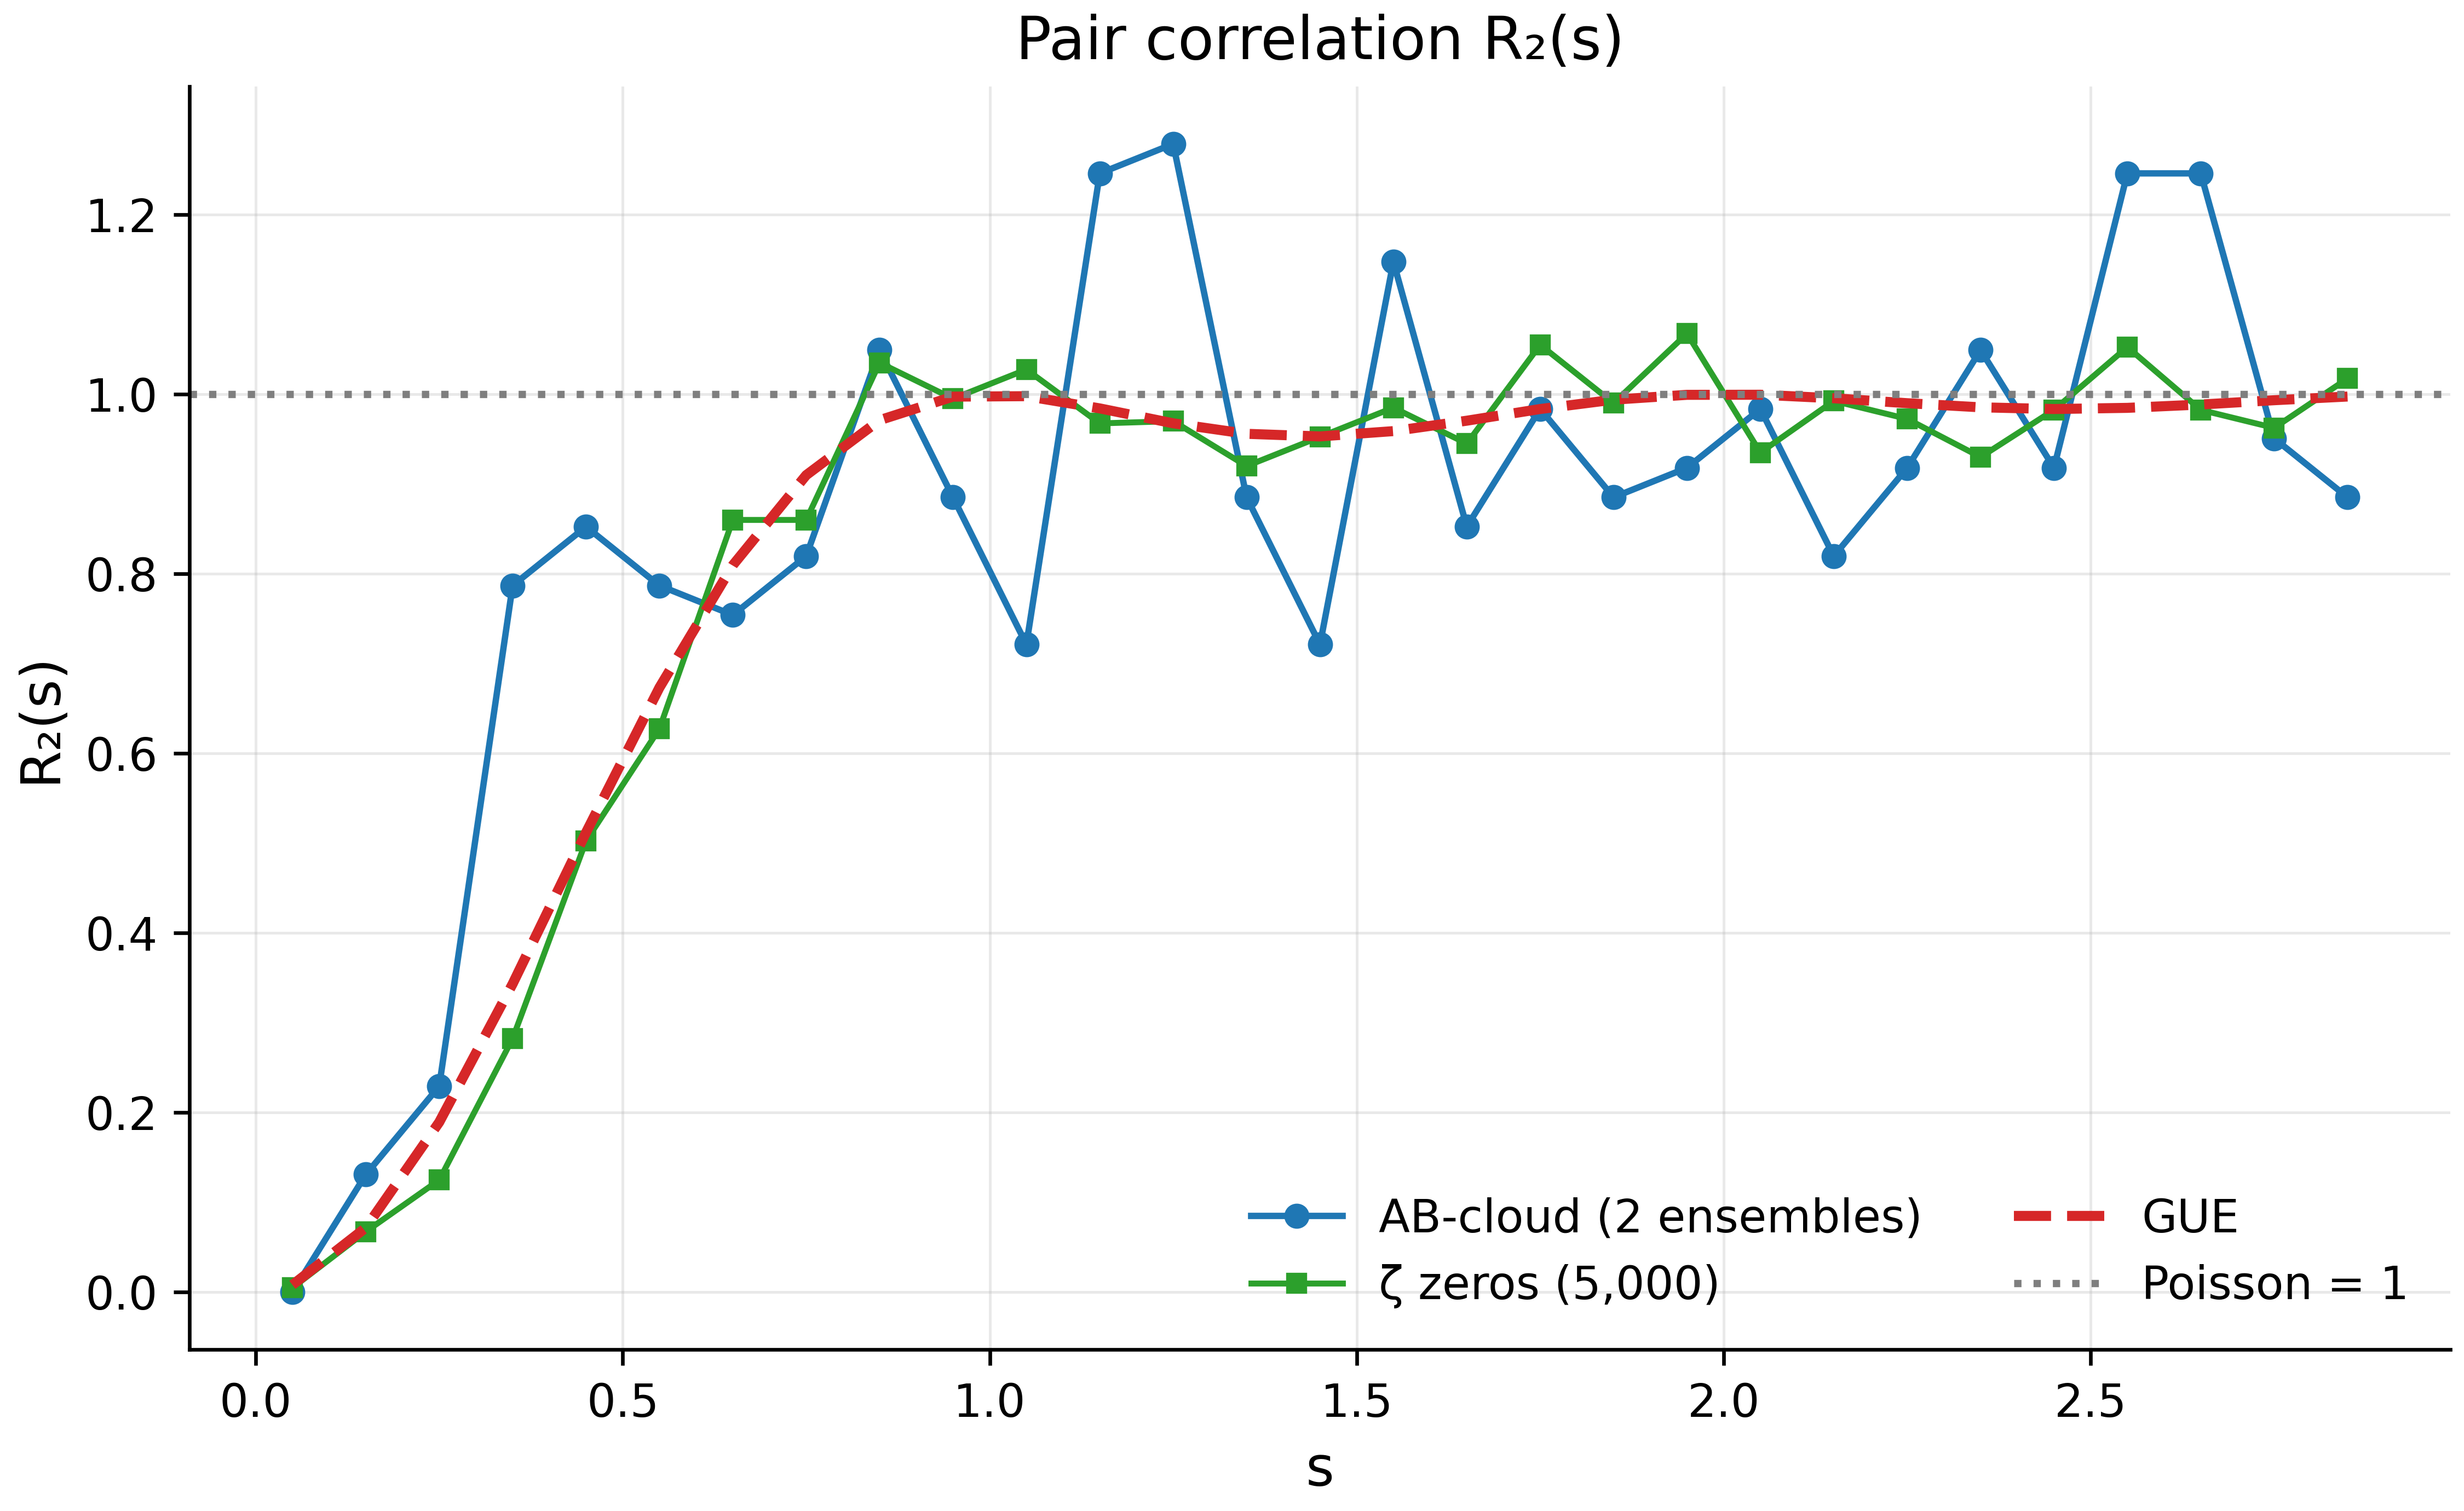
\includegraphics[width=0.72\textwidth]{../../figures/fig08_r2_pair.png}
\caption{Pair correlation $R_2(s)$: the AB-cloud against the $\zeta$ zeros, GUE and Poisson (Test 35).}
\end{figure}

\section{Dirac Dynamics and the Critical Line}
$E_{\min}=0.0202+11.826/L$ with $R^2=0.9997$ over $L=12\dots48$ (four zero modes at every size); $v_F=b/2\pi\approx1.88$ for a Dirac point at the zone center. The DOS dip at $\alpha=1/2$: $\rho=0.010$ against $0.200$ at $\alpha=0.4/0.6$ --- a $20\times$ contrast. For $\sigma\ne1/2$ (the phase generalization) the spectrum becomes fully complex (max $|\mathrm{Im}\,E|=0.623$ at $\sigma=0.7$), with skin parameter $g=0.322$: the critical line $\sigma=1/2$ is the only line of bulk random-matrix statistics, consistent with its role as the Connes self-dual point.

\section{Analytic Structures}
Exact identities (machine precision): $\Phi_{AB}=2\pi/14=\pi/7$ for $q/e=1/14$; $\gamma^\ast=a_C+ib_C$ with $a_C=(\pi/7)^5/22=8.276\cdot10^{-4}$, $b_C=2\sin^2(\pi/7)=0.3765$, argument $89.874^\circ\approx\pi/2$; the complex fractal factor $CF=\exp(2\pi i/22)\exp(i\beta\ln22)$, $\beta=2.854$, $|CF|=1$, with the empirical input $CF_{\rm hard}$ and $c_{AB}=0.0206$. Status: the formulas are exact; their physical interpretation (a Peccei--Quinn phase, the PSL$(2,7)\subset M$ Moonshine) remains hypothetical.

\section{Conclusion}
The AB-cloud is a phase resonator with reproducible GUE statistics, an exact topological skeleton, and Dirac low-energy dynamics; its correlations match those of the $\zeta$ zeros at the level of universality, and the discrepancies are quantitatively explained by finite size. All numbers are reproducible by commands from the repository; every test leaves full logs and reports.

\begin{thebibliography}{9}
\bibitem{montgomery} H.~L. Montgomery, \emph{The pair correlation of zeros of the zeta function}, Proc. Sympos. Pure Math. \textbf{24}, 181 (1973).
\bibitem{odlyzko} A.~M. Odlyzko, \emph{On the distribution of spacings between zeros of the zeta function}, Math. Comp. \textbf{48}, 273 (1987).
\bibitem{berry} M.~V. Berry, \emph{Semiclassical formula for the number variativity of the Riemann zeros}, Nonlinearity \textbf{1}, 151 (1988); M.~V. Berry, in \emph{Quantum Chaos and Statistical Nuclear Physics}, Springer (1986).
\bibitem{hofstadter} D.~R. Hofstadter, \emph{Energy levels and wave functions of Bloch electrons in rational and irrational magnetic fields}, Phys. Rev. B \textbf{14}, 2239 (1976).
\bibitem{byers} N. Byers, C.~N. Yang, \emph{Theoretical considerations concerning quantum electromagnetic fields in the presence of superconductors}, Phys. Rev. Lett. \textbf{7}, 46 (1961).
\bibitem{fukui} T. Fukui, Y. Hatsugai, H. Suzuki, \emph{Chern numbers in discretized Brillouin zone}, J. Phys. Soc. Jpn. \textbf{74}, 1674 (2005).
\bibitem{dyson} F.~J. Dyson, \emph{The threefold way}, J. Math. Phys. \textbf{3}, 1199 (1962).
\bibitem{hatano} N. Hatano, D.~R. Nelson, \emph{Localization resonances and loss coefficients in non-Hermitian models}, Phys. Rev. B \textbf{56}, 8651 (1997).
\bibitem{tknn} D.~J. Thouless, M. Kohmoto, M.~P. Nightingale, M. den Nijs, \emph{Quantized Hall conductance in a two-dimensional periodic potential}, Phys. Rev. Lett. \textbf{49}, 405 (1982).
\bibitem{berrykeating} M.~V. Berry, J.~P. Keating, \emph{$H=xp$ and the Riemann zeros}, SIAM Review \textbf{41}, 236 (1999).
\end{thebibliography}

\end{document}
